\begin{frame}\frametitle{Jets$\rightarrow \gamma$ Background. Sources}
  \scriptsize
  Jets$\rightarrow \gamma$ background estimation is the most challenging part of this measurement and also the source of the largest systematic uncertainties (discussed later).
\end{frame}

\begin{frame}\frametitle{Jets$\rightarrow \gamma$ Background. Template Method}
  \scriptsize
  \begin{itemize}
    \item Fit function: $F(V_{fit})=N_{true} \cdot T_{true}(V_{fit}) + N_{fake} \cdot T_{fake}(V_{fit})$
%    \item $V_{fit}=I_{ch}^{\gamma}$ and $V_{fit}=\sigma_{i\eta{i\eta}}$ are considered
%    \item $T_{true}$: Real-$\gamma$ template from Z$\gamma\rightarrow\mu\mu\gamma$ FSR minus [small] fake contamination based on DYjets MC
%    \item $T_{fake}$: Fake-$\gamma$ template from Z$\gamma\rightarrow\mu\mu\gamma$ ISR minus [large] real contamination based on Z$\gamma$ MC
%    \item For $I_{ch}$, real-$\gamma$: use full data $p_T^{\gamma}>15~GeV$, fake-$\gamma$: use data only for certain $p_T^{\gamma}$ to prepare template;
%    \item For $\sigma_{i\eta{i\eta}}$, real-$\gamma$: merge data for $p_T^{\gamma}>30~GeV$ for preparing templates, fake-$\gamma$: merge data for $p_T^{\gamma}>55~GeV$;
%    \item Same templates for the muon and the electron channels;
%    \item Algorithm of template rebinning is applied if necessary;
%    \item After fit is performed, extract $N_{real}=\epsilon_{real} \cdot N_{real}^{from-fit}$,  $N_{fake}=\epsilon_{fake} \cdot N_{fake}^{from-fit}$, where $\epsilon_{real}$($\epsilon_{fake}$) is efficiency of real-$\gamma$(fake-$\gamma$) events to pass the nominal cut of $V_{fit}$ computed from the Z$\gamma$ FSR sample (Z$\gamma$ ISR data and MC samples).
  \end{itemize}
\end{frame}

\begin{frame}\frametitle{Jets$\rightarrow \gamma$ Background. Templates from $Z\gamma\rightarrow{\bar{\mu}}\mu\gamma$}
  \begin{figure}[htb]
    \begin{center}
       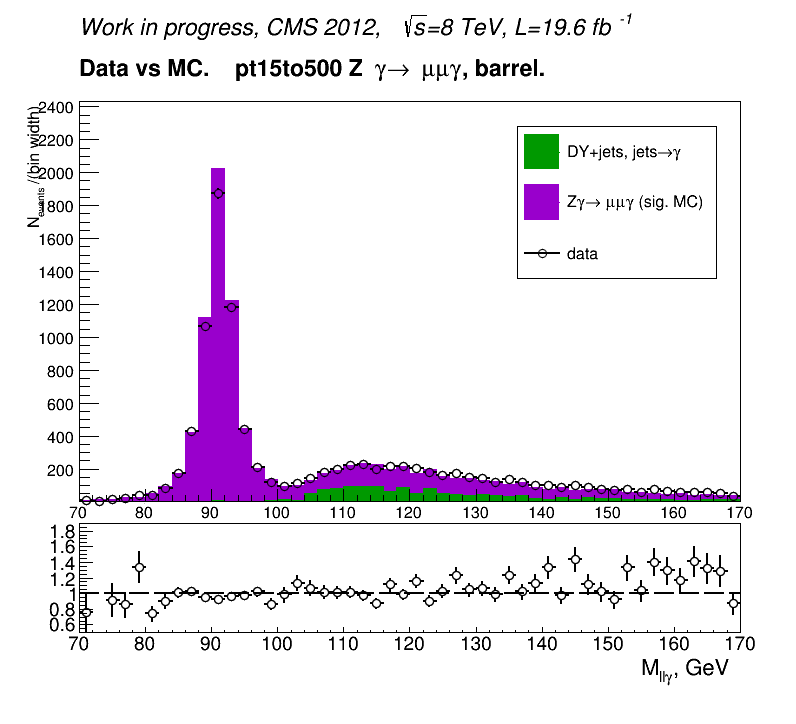
\includegraphics[width=0.25\textwidth]{../figs/figs_v11/MUON_ZGamma/PrepareYields/c_TotalDATAvsMC_Barrel__MpholeplepVERY_PRELIMINARY_pt15to500_.png}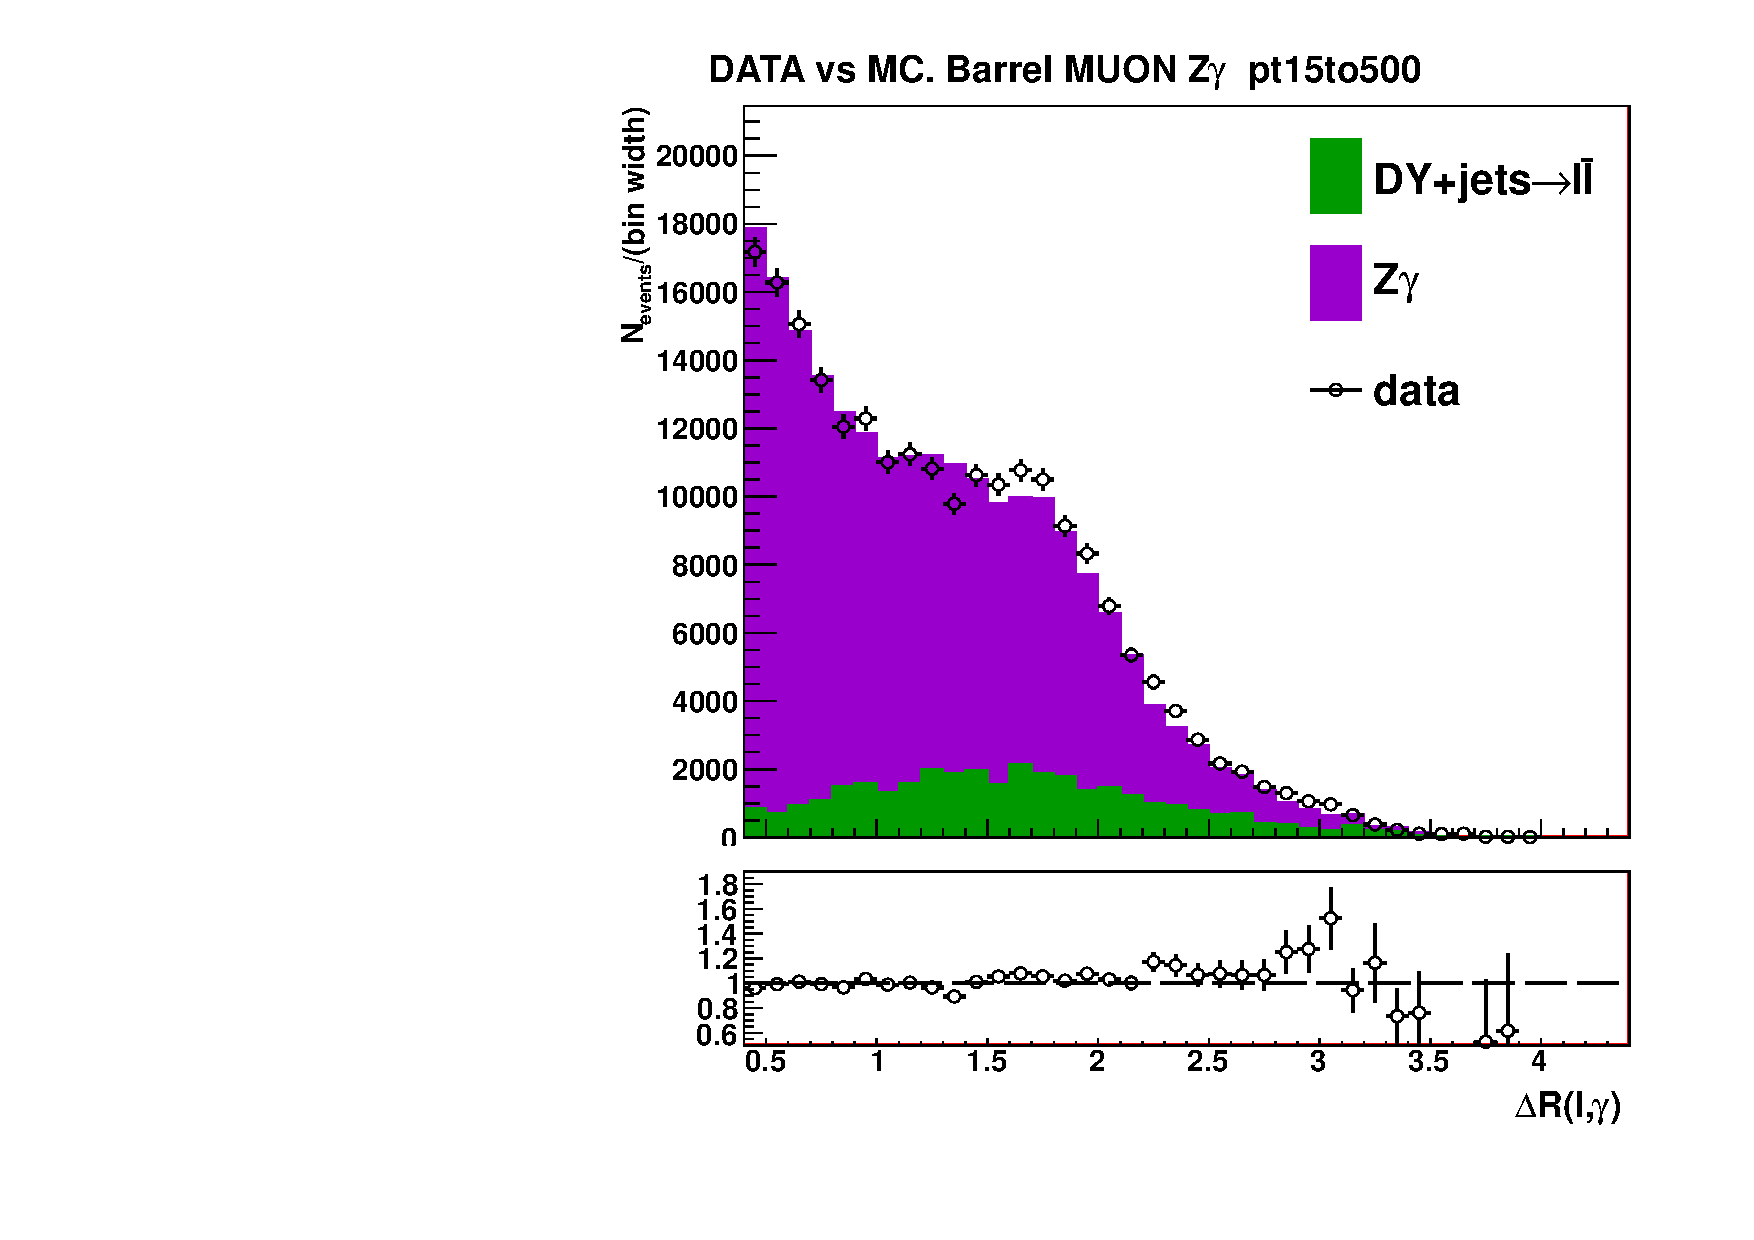
\includegraphics[width=0.25\textwidth]{../figs/figs_v11/MUON_ZGamma/PrepareYields/c_TotalDATAvsMC_Barrel__lep1PhoDeltaRVERY_PRELIMINARY_pt15to500_.pdf}\\
% 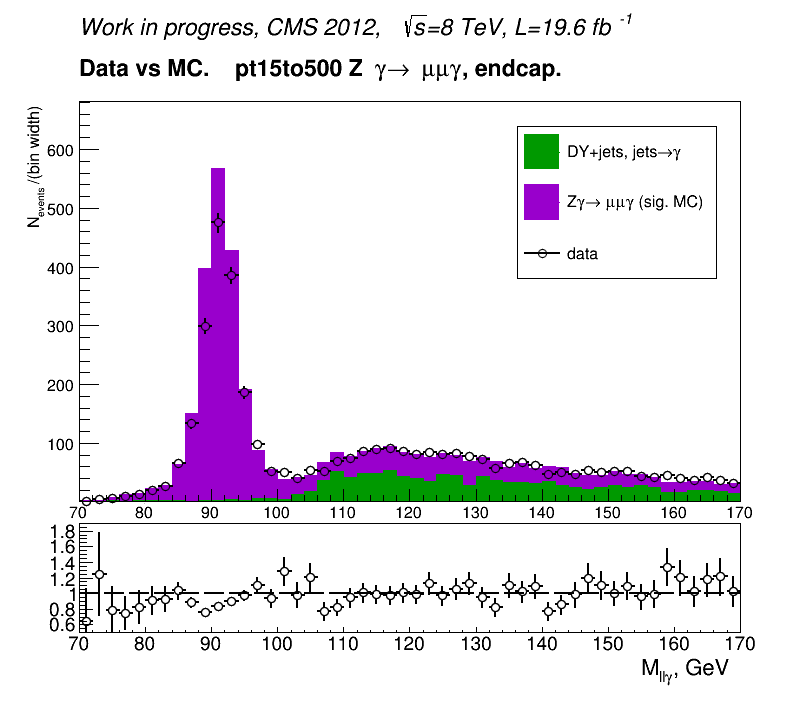
\includegraphics[width=0.40\textwidth]{../figs/figs_v11/MUON_ZGamma/PrepareYields/c_TotalDATAvsMC_Endcap__MpholeplepVERY_PRELIMINARY_pt15to500_.png}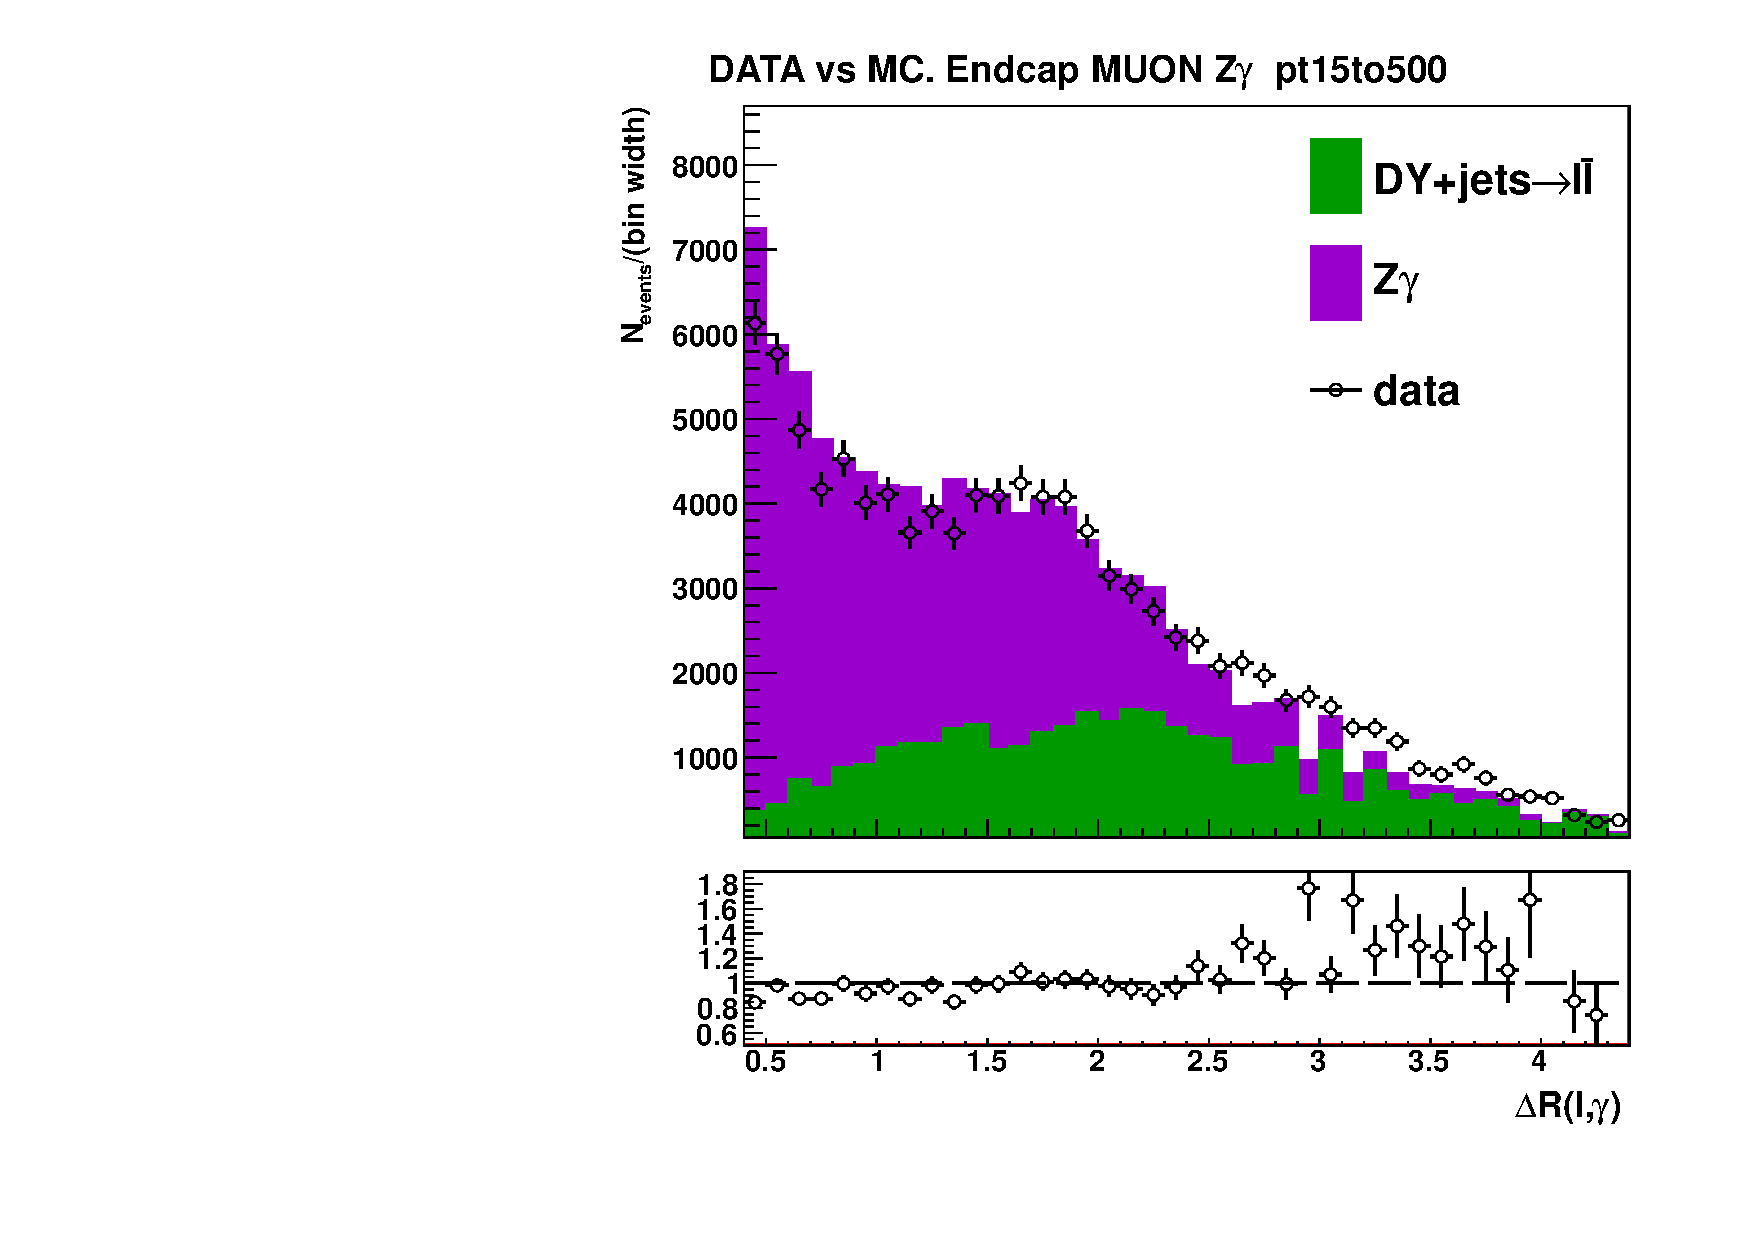
\includegraphics[width=0.40\textwidth]{../figs/figs_v11/MUON_ZGamma/PrepareYields/c_TotalDATAvsMC_Endcap__lep1PhoDeltaRVERY_PRELIMINARY_pt15to500_.pdf}
    \end{center}
  \end{figure}
\scriptize
FSR selection: $M_{\mu\mu\gamma}<101$~GeV and $\Delta R(\mu_{1},\gamma)>0.4$\\
ISR selection: $M_{\mu\mu\gamma}>101$~GeV and $\Delta R(\mu_{1},\gamma)>1.0$
\end{frame}%{{Jets$\rightarrow \gamma$ Background. Templates from $Z\gamma\rightarrow{\bar{\mu}}\mu\gamma$}

\begin{frame}\frametitle{$Jets \rightarrow \gamma$ Background. $V_{fit}=I_{ch}^{\gamma}$ and $V_{fit}=\sigma_{i\eta{i\eta}}$}
  \begin{figure}[htb]
    \begin{center}
       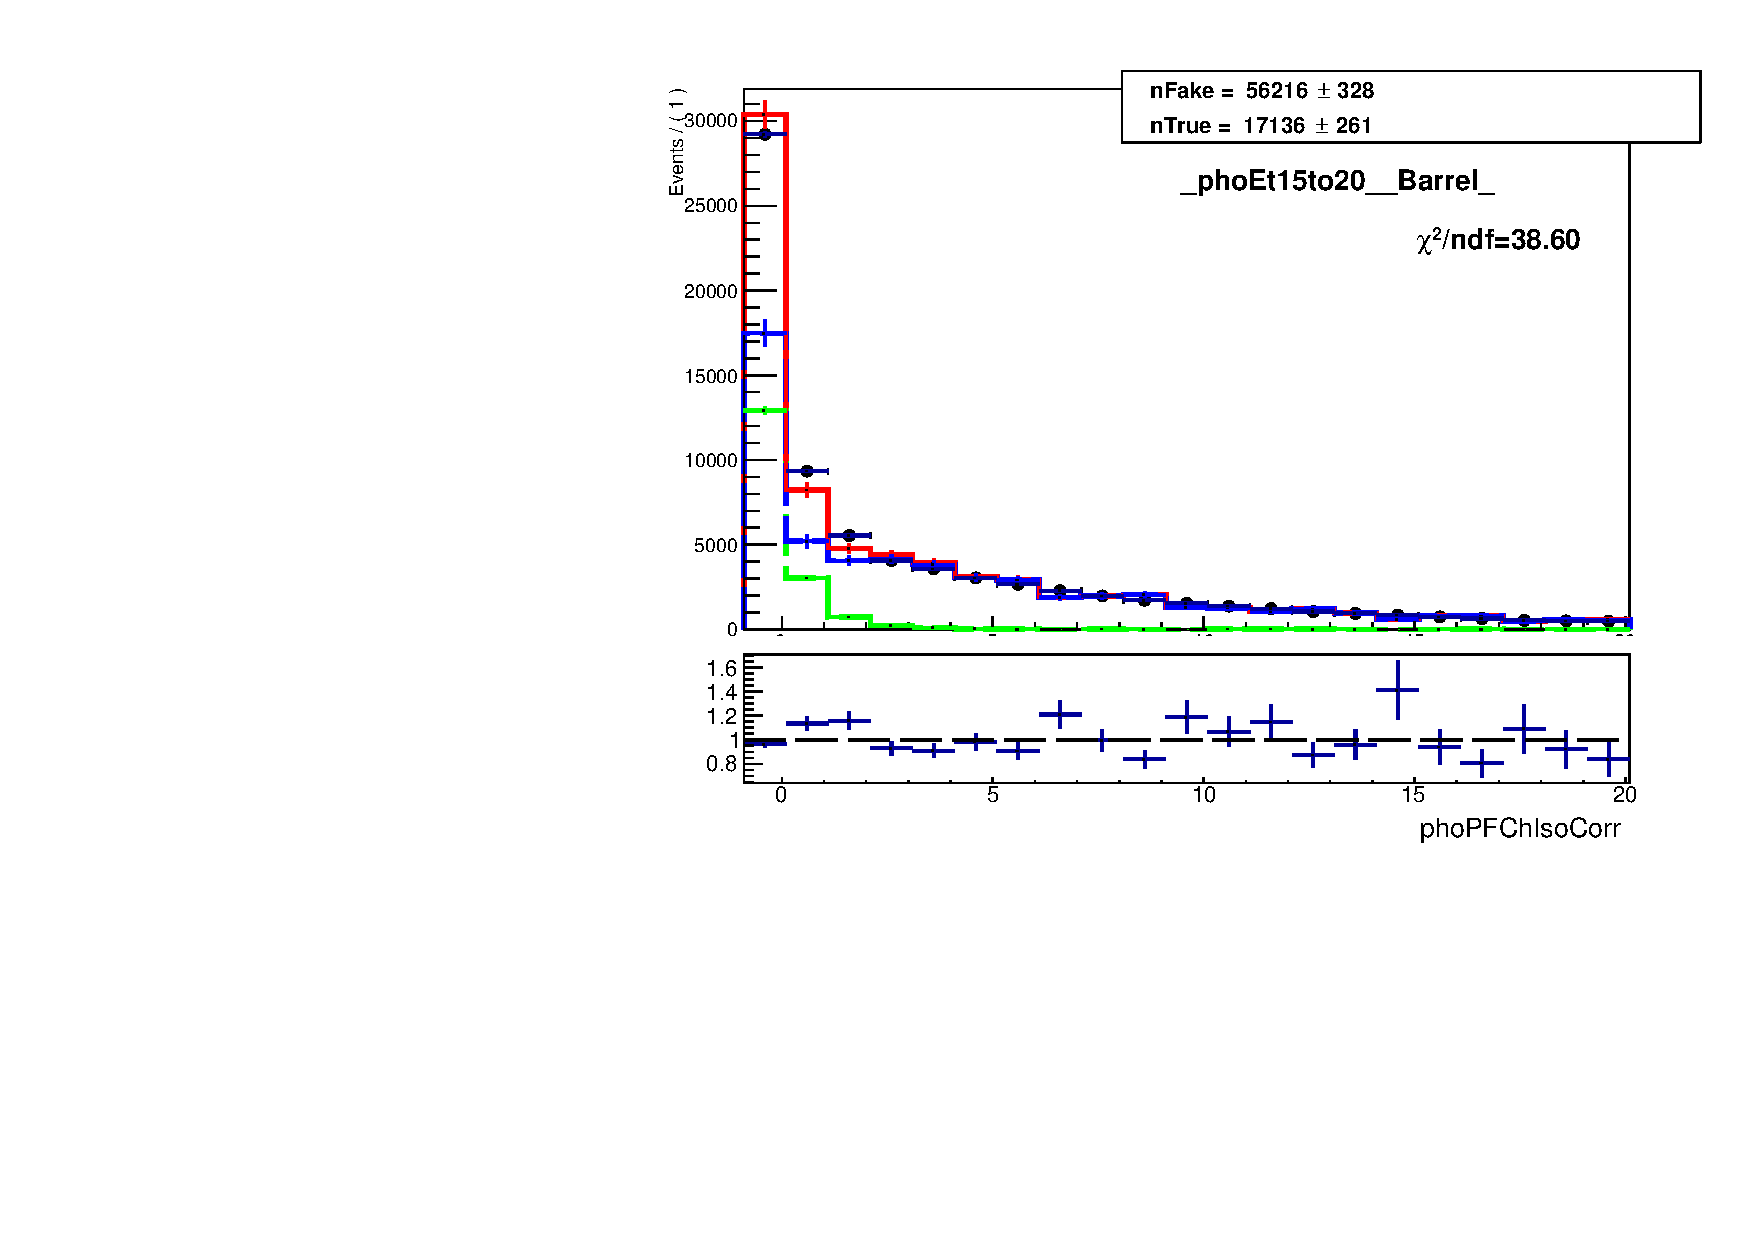
\includegraphics[width=0.25\textwidth]{../figs/figs_v11/MUON_WGamma/TemplateFits/c_TEMPL_CHISO_UNblind__phoEt15to20__Barrel__RooFit.pdf} 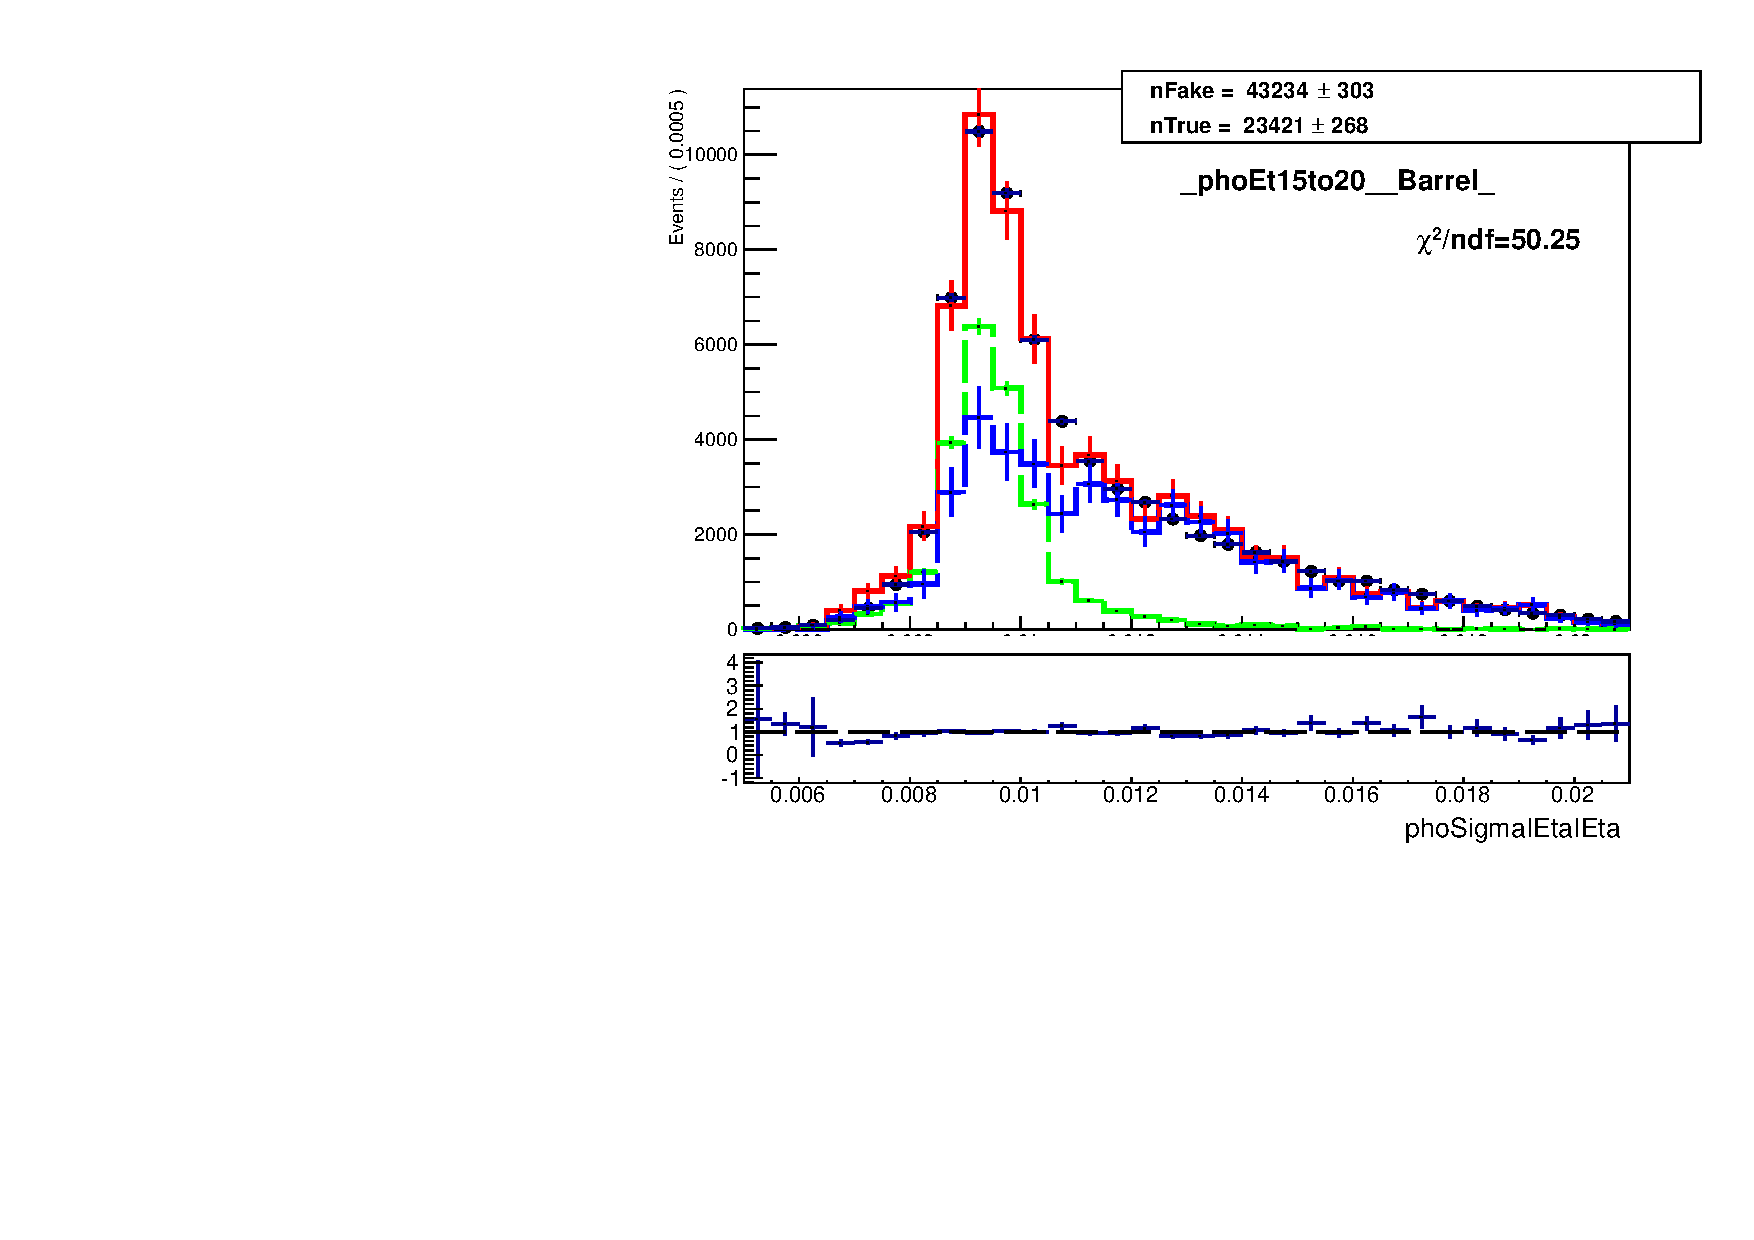
\includegraphics[width=0.45\textwidth]{../figs/figs_v11/MUON_WGamma/TemplateFits/c_TEMPL_SIHIH_UNblind__phoEt15to20__Barrel__RooFit.pdf}
    \end{center}
  \end{figure}
\end{frame}%{$Jets \rightarrow \gamma$ Background Subtraction. $V_{fit}=I_{ch}^{\gamma}$}
